By construction, $E_{proj}$ is always very close to zero at the end of the execution (the algorithm come closer and closer to the feasible space).\\
Fig. \ref{fig:eproj}. illustrates this behavior on a tipical example : 
\begin{figure}[h]
	\label{fig:eprojexample}
	\caption{Evolution of $E_{proj}$ during a tipical execution}
	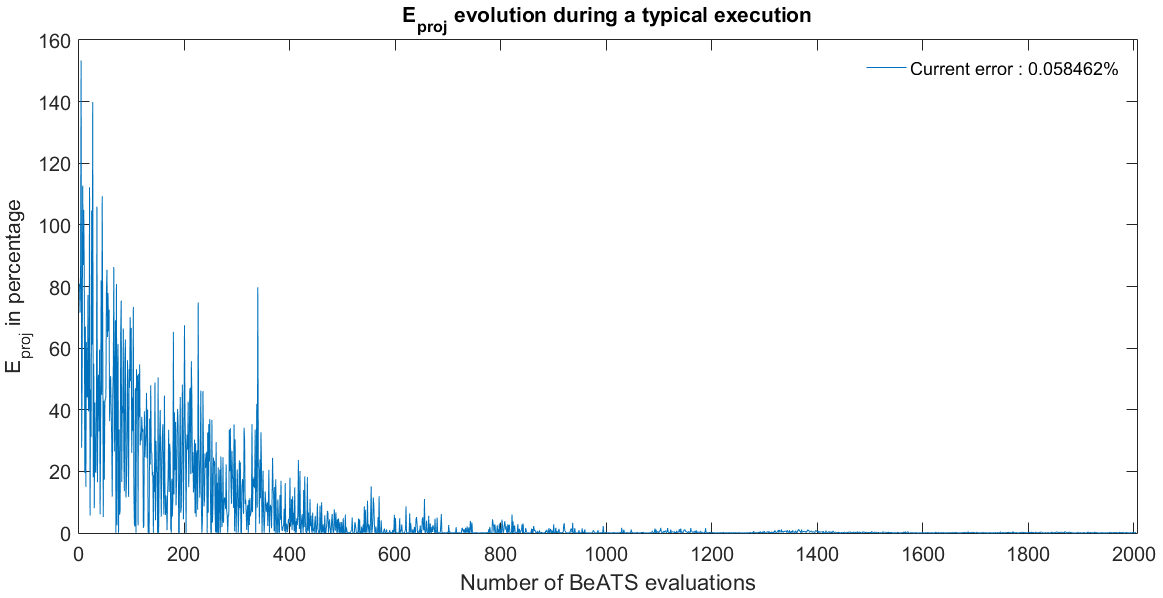
\includegraphics[width=7in]{figures/results_figures/eprojexample.png}
\end{figure}	
By imputation, as explained in \ref{subsec:vmt} and \ref{subsec:implementation}, $E_VMT$ is always below $5\%$, often around $2\%$, on each iteration of the algorithm.\\
Fig. \ref{fig:tvmexample} reflects the history of $VMT$ during a tipical run.
\begin{figure}[h]
	\label{fig:vmtexample}
	\caption{Evolution of $VMT$ during a tipical execution}
	\includegraphics[width=7in]{figures/results_figures/vmtexample.png}
\end{figure}	
VHT is quite correlated with the congestion : on most executions, that lead to an acceptable congestion, $E_{TVH}^{*}$ is less than $U^{global}=5\%$. However, particularly when the knobs are constrained too much,  $E_{TVH}^{*}$ ends up around $20\%$.
Fig. \ref{fig:tvhexample} reflects the history of $VHT$ with its most common behavior.
\begin{figure}[h]
	\label{fig:vhtexample}
	\caption{Evolution of $VHT$ during a tipical execution}
	\includegraphics[width=7in]{figures/results_figures/vhtexample.png}
\end{figure}	

